%
% $RCSfile: encapsulation.tex,v $
%
% Copyright (C) 2002-2008. Christian Heller.
%
% Permission is granted to copy, distribute and/or modify this document
% under the terms of the GNU Free Documentation License, Version 1.1 or
% any later version published by the Free Software Foundation; with no
% Invariant Sections, with no Front-Cover Texts and with no Back-Cover
% Texts. A copy of the license is included in the section entitled
% "GNU Free Documentation License".
%
% http://www.cybop.net
% - Cybernetics Oriented Programming -
%
% http://www.resmedicinae.org
% - Information in Medicine -
%
% Version: $Revision: 1.1 $ $Date: 2008-08-19 20:41:06 $ $Author: christian $
% Authors: Christian Heller <christian.heller@tuxtax.de>
%

\subsubsection{Encapsulation}
\label{encapsulation_heading}
\index{Encapsulation}
\index{Access Method}
\index{Java}
\index{Information Hiding}
\index{Data Hiding}
\index{public}
\index{protected}
\index{private}
\index{Delphi}
\index{published}

One recommendation of object oriented programming is that the properties of an
object created as instance of a class be protected through special
\emph{Access Methods} (figure \ref{encapsulation_figure}). A \emph{Java} code
example can be found below. The intention is not to expose class attributes to
other classes by minimising direct access to them and such to provide some
security by preventing illegal access to an object's interna. Therefore, this
paradigm is called \emph{Encapsulation} or \emph{Information-/ Data Hiding}.
Another advantage is that if an attribute changes its name, then only one place
in the code (the access method), instead of hundreds, needs to be updated.

\begin{scriptsize}
    \begin{verbatim}
    public class example_class {
        private Type attribute;
        public void set_attribute(Type a) {
            this.attribute = a;
        }
        public Type get_attribute() {
            return this.attribute;
        }
    }
    \end{verbatim}
\end{scriptsize}

\begin{figure}[ht]
    \begin{center}
        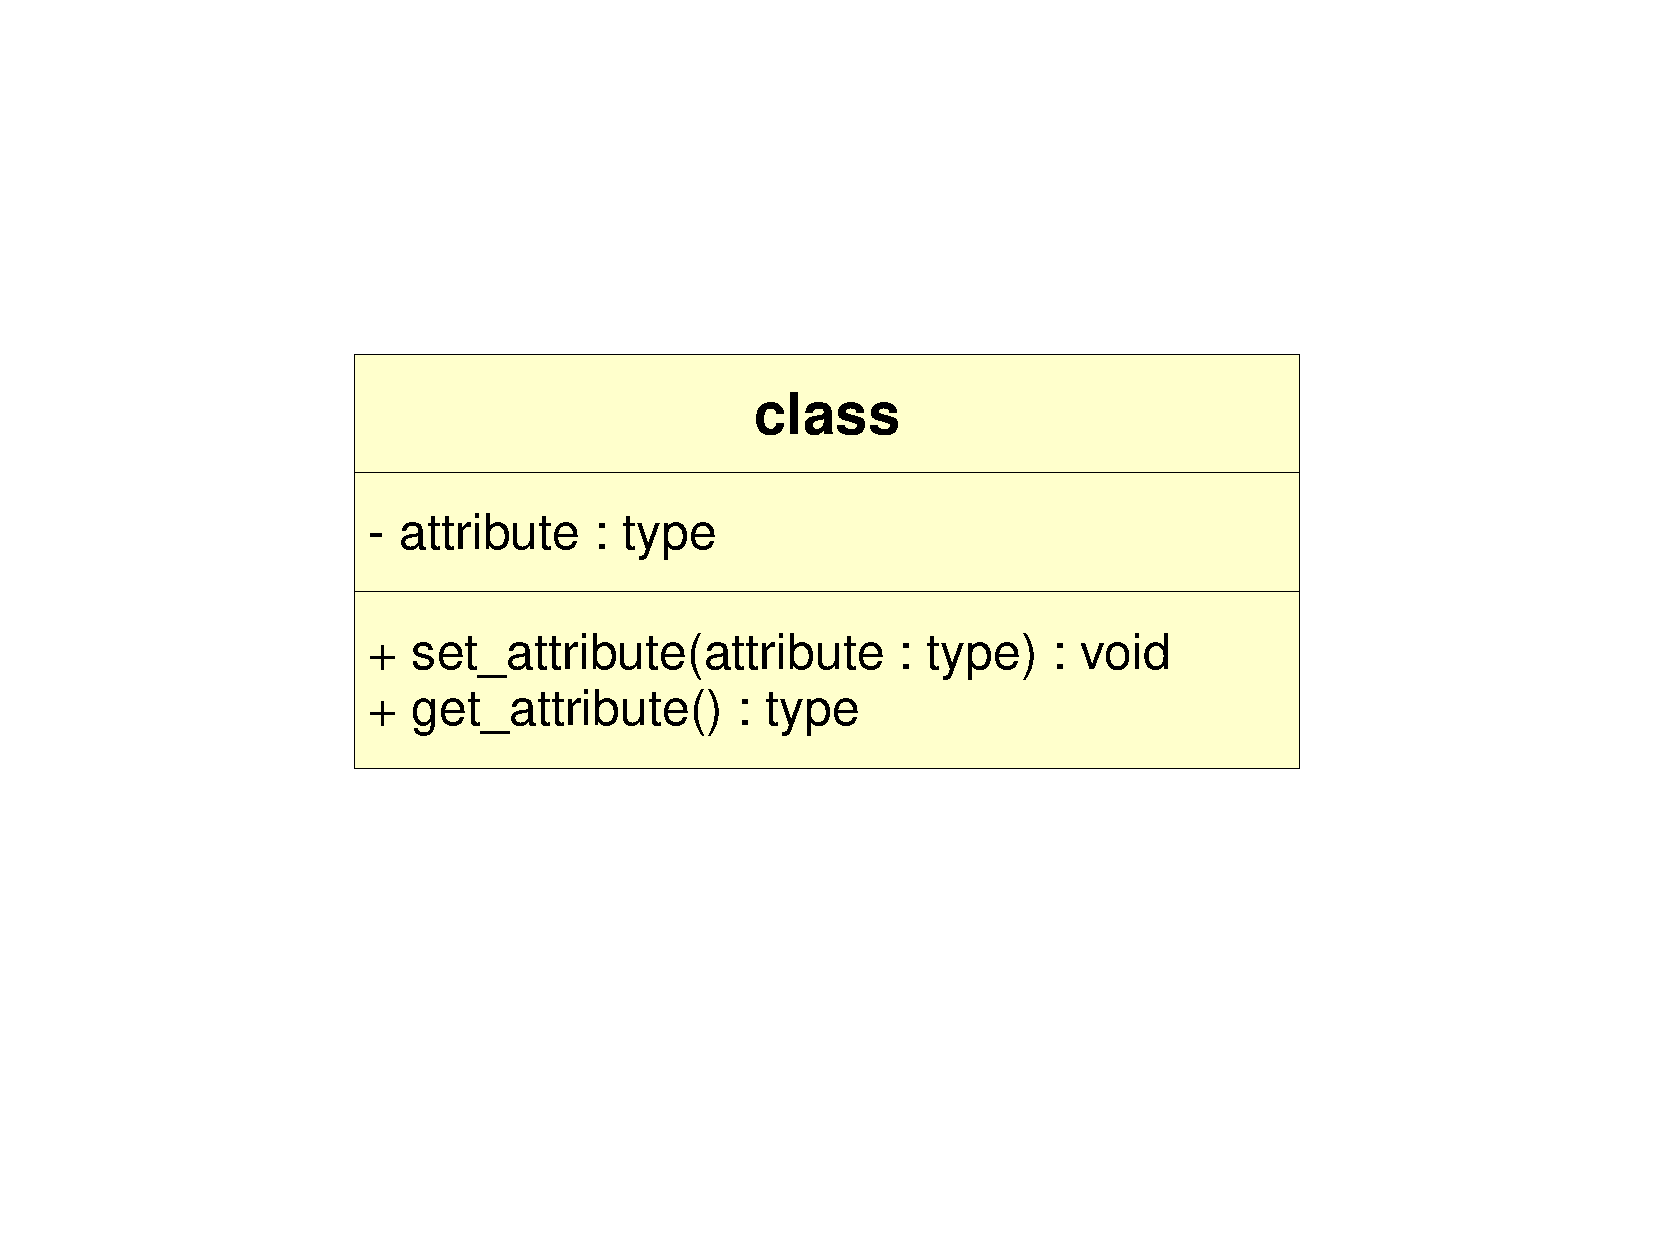
\includegraphics[scale=0.3,angle=-90]{graphic/encapsulation.pdf}
        \caption{Encapsulation as UML Diagram}
        \label{encapsulation_figure}
    \end{center}
\end{figure}

Special keywords are necessary to ensure proper encapsulation by making
attributes and methods \emph{visible} to only certain outside objects. These
keywords are: \emph{public}, \emph{protected} and \emph{private}. In the
\emph{Java} programming language \cite{java}, an additional package protection
level is applied when none of the aforementioned keywords is found. The
\emph{Delphi} language \cite{warken} knows an additional \emph{published}
keyword that makes properties visible in its object-inspector tool. Other
languages may contain further variations of access limitations.

The recommendation to encapsulate attributes produces thousands of lines of
source code whose usefulness is at least questionnable \cite{hellerbohl}. In
about 90\% of cases (practical experience of the author of this document), the
\emph{set} and \emph{get} methods consist of only one single line accessing an
attribute value which in the end is the same as accessing that attribute
directly. Sometimes, additional lines with a trigger function to update other
parts of the system are added. They get invoked whenever an attribute value of
the called object is changed by a \emph{set} method:

\begin{scriptsize}
    \begin{verbatim}
    public void set_attribute(Type a) {
        this.attribute = a;
        get_update_manager().update(this);
    }
    \end{verbatim}
\end{scriptsize}

But, as shown below, this update notification could as well be taken over by
the object that was calling the \emph{set} method:

\begin{scriptsize}
    \begin{verbatim}
    public void method() {
        example_object.set_attribute(a);
        get_update_manager().update(example_object);
    }
    \end{verbatim}
\end{scriptsize}

The argumentation that \textit{in this case a lot of redundant code would be
produced since the update function has to be implemented in every calling
object, instead of just once in the called object} does not really hold true
when looking into programming practice. The number of external objects calling
an object is mostly very well manageable. It finally seems that thousands of
\emph{set}/ \emph{get} access methods could be eliminated which would lead to a
tremendous code reduction and improved clearity.

The language introduced in chapter \ref{cybernetics_oriented_language_heading}
does not use encapsulation and the attributes (state knowledge) and methods
(logic knowledge) modelled in it are not bundled together.
